% \documentclass{article}
\documentclass[11pt]{article}
\usepackage{graphicx}
\usepackage{hyperref}
\usepackage{caption}



\newcommand{\numpy}{{\tt numpy}}    % tt font for numpy

\topmargin -.5in
\textheight 9in
\oddsidemargin -.25in
\evensidemargin -.25in
\textwidth 7in

\begin{document}

% ========== Edit your name here
\author{Hongqing Liu, hl85}
\title{CS 498: Assignment 1: Perspective Projection}
\date{February 7, 2023}
\maketitle

\medskip


\section*{Submission}

In this assignment you will be modifying the files homography.py and perspective.py.
Please put together a single PDF with your answers and figures for each problem, and submit to Gradescope (Course Code: BBX6NE). We recommend you to add your answers to the latex template files we provided. For code submission, make sure you use the provided ".py" files with your modification and the dumped ``.npz'' file. The graders will check both your PDF submission and your code submission if needed. 


\section*{Homography [8pts]}

In this question, we will examine properties of homography transformations and see how to estimate a planar homography from a set of correspondences. 

\paragraph{Question 1 [1pt]:} You are given a photo of the State Farm Center (\texttt{uiuc.png}), UIUC's indoor arena that hosts our basketball teams. We marked and plotted the four corners of the court, as shown in Fig.~\ref{fig:intro} (left). A standard basketball court is 28.65 meters long and 15.24 meters wide, as shown in Fig.~\ref{fig:intro} (right). Now let's consider a 2D coordinate system defined on the planar surface of the basketball court. The origin of this coordinate system is point \#3; the long edge is x axis and short edge is y axis. Please write down the four corner's coordinates in this 2D coordinate frame (in meters) and fill in your answer in the numpy array ``corners\_court". 

\begin{figure}[htbp]
\small
\includegraphics[width=0.48\linewidth]{goillini.png}
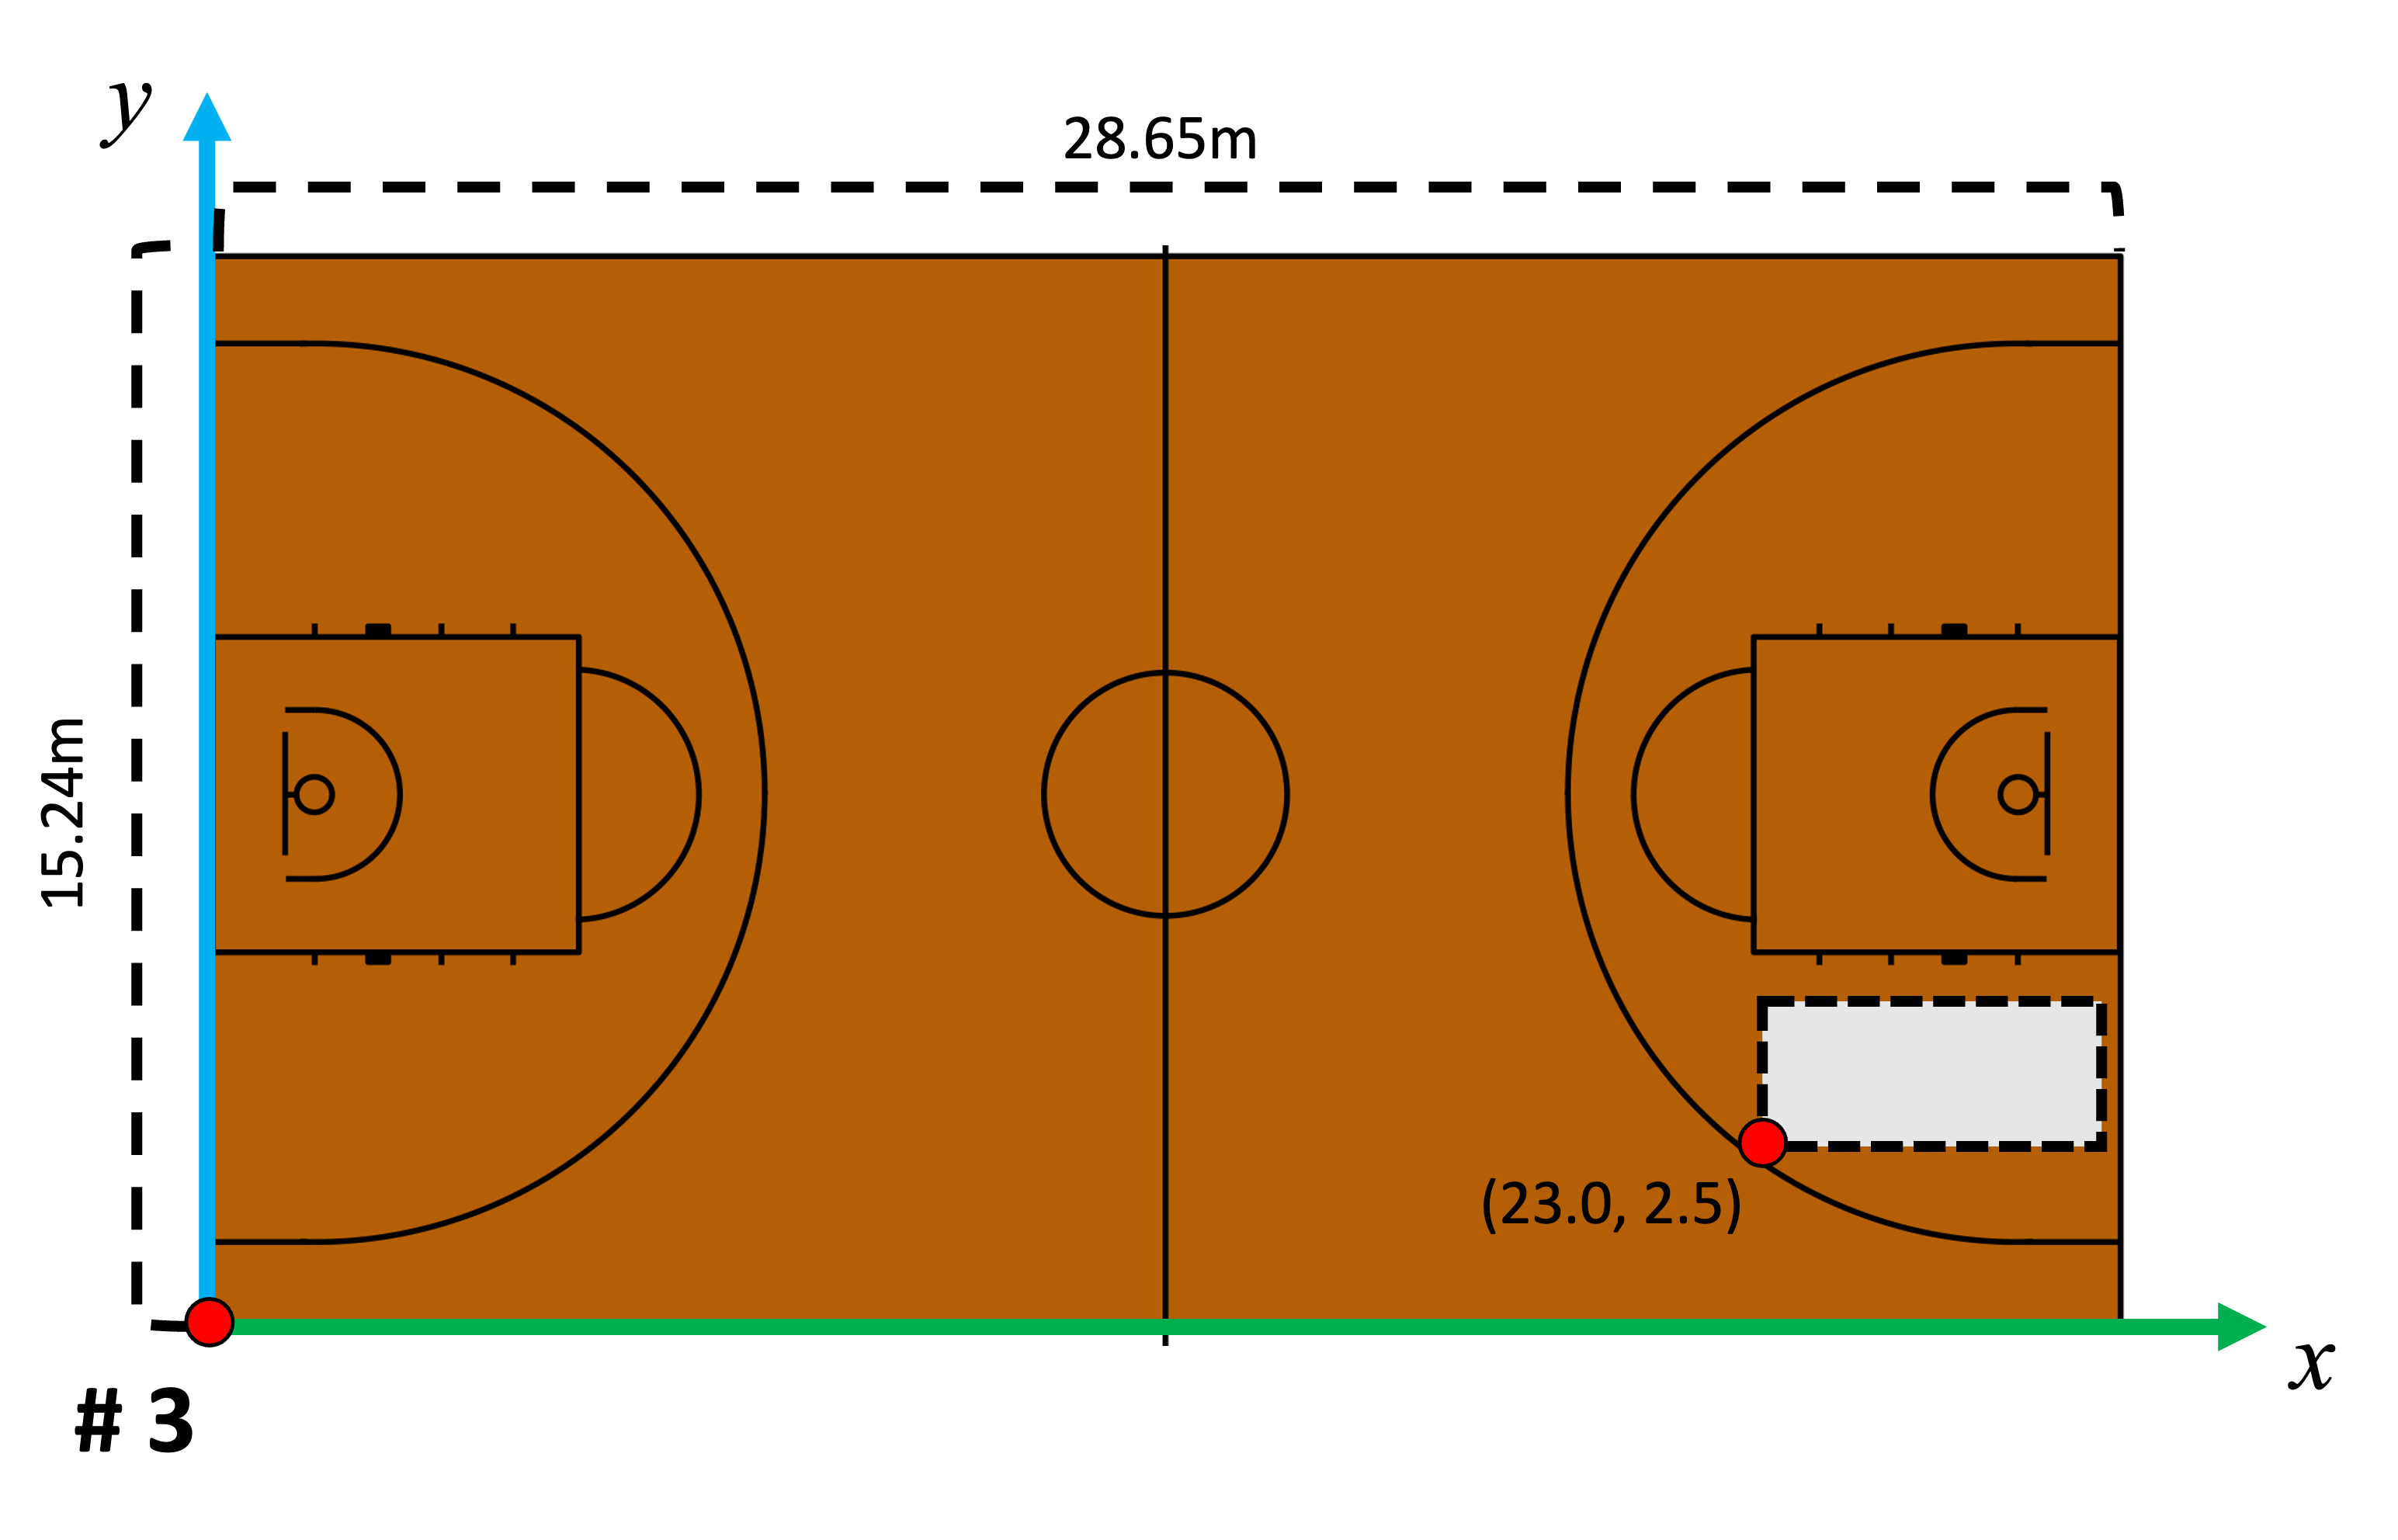
\includegraphics[width=0.5\linewidth]{coordinate.png}
\caption{ Left: target image with keypoints; Right: court dimensions and coordinate convention.}
\label{fig:intro}
\end{figure}

\textbf{Answer}:  The four coner's coordinates are point0$(0,15.24)$, point1$(28.65,15.24)$, point2($28.65,0)$, point3$(0,0)$. 
\[
conersCourt = 
\left[
\begin{array}{cc}
0 & 15.24 \\
28.65 & 15.24 \\
28.65 & 0 \\
0 & 0 \\
\end{array}
\right]
\]
\paragraph{Question 2 [3pts]:}
Given your Q1's answer, now we could establish four pairs of point correspondence between two planes: the 2D basketball court plane and the 2D image plane. Using what we have learned in Lecture 3, complete the function \texttt{findHomography} and use it to estimate the homography matrix from the court to the image. Please briefly explain what you do for homography estimation and report the resulting matrix in this document. Hints: 1) you might find the functions \texttt{vstack, hstack} to be handy for getting homogenous coordinates; 2) you might find \texttt{numpy.linalg.svd} to be useful; 3) lecture 3 described the homography estimation process. 

\textbf{Answer}: 

Since we want to project a 3D object into a 2D image, we can transform the 3D coordinate into 2D by a projection matrix. Here we use homogeneous world coordinates(4x1) and homogeneous image coordinates(3x1), as shown below. The last item in image coordinates z shows the scalar ambiguity.
\[
\left[
\begin{array}{c}
x \\
y \\
z
\end{array}
\right] = 
\left[
\begin{array}{cccc}
p_1 & p_2 & p_3 & p_4 \\
p_5 & p_6 & p_7 & p_8 \\
p_9 & p_{10} & p_{11} & p_{12} \\
\end{array}
\right]
\left[
\begin{array}{c}
X \\
Y \\
Z \\
1
\end{array}
\right]
\]

Since the basketball court plane is in a 2D coordinate, which means it is a planar object and its z-coordinate is always 0. In that case, $p_3$, $p_7$ and $p_11$ has no attribute to xyz 2D image coordinate.

Since we know that x and PX have same orientation, their cross product will equal 0, as shown below:

\begin{equation}
x = kPX \rightarrow \vec{x} \times \vec{PX} = 0
\end{equation}

Each pairs of corresponding points can establish 2 equations, since the P[3,3] needs to be 1, we need a eight-simultaneous equations to find the solution, which means we need four pairs of corresponding points. The equation systems can be wirtten in the form of matrix multiplication, as follows.

\[
\left[
\begin{array}{ccccccccc}
0 & 0 & 0 & X_1 & Y_1 & 1 & -y_1^\prime X_1 & -y_1^\prime Y_1 & -y_1^\prime \\
X_1 & Y_1 & 1 & 0 & 0 & 0 & -x_1^\prime X_1 & -x_1^\prime Y_1 & -x_1^\prime \\
0 & 0 & 0 & X_2 & Y_2 & 1 & -y_2^\prime X_2 & -y_2^\prime Y_2 & -y_2^\prime \\
X_2 & Y_2 & 1 & 0 & 0 & 0 & -x_2^\prime X_2 & -x_2^\prime Y_2 & -x_2^\prime \\
0 & 0 & 0 & X_3 & Y_3 & 1 & -y_3^\prime X_3 & -y_3^\prime Y_3 & -y_3^\prime \\
X_3 & Y_3 & 1 & 0 & 0 & 0 & -x_3^\prime X_3 & -x_3^\prime Y_3 & -x_3^\prime \\
0 & 0 & 0 & X_4 & Y_4 & 1 & -y_4^\prime X_4 & -y_4^\prime Y_4 & -y_4^\prime \\
X_4 & Y_4 & 1 & 0 & 0 & 0 & -x_4^\prime X_4 & -x_4^\prime Y_4 & -x_4^\prime \\
\end{array}
\right]
\left[
\begin{array}{c}
h_1 \\
h_2 \\
h_3 \\
h_4 \\
h_5 \\
h_6 \\
h_7 \\
h_8 \\
h_9
\end{array}
\right] = \mathbf{0}
\]

After that, I form a matrix A from the set of correspondences, each row of the matrix corresponds to a single correspondence. After that, I perform SVD on the matrix A to obtain its singular values and singular vectors. The last column of the right singular vector corresponding to the smallest singular value represents the entries of the projection matrix. After that, I resized it into 3x4 and normalized the projection matrix by divde it by its last element.

The projection matrix is shown as follows:

\[ P = 
\left[
\begin{array}{ccc}
1.20809640e+01 & 4.44696370e+01 & 7.92073117e+01 \\
-8.05770293e+00 & 5.76174339e+00 & 6.42252451e+02 \\
-2.12530603e-02 & 1.65326163e-02 & 1.00000000e+00 \\
\end{array}
\right]
\]

\paragraph{Question 3 [4pts]:}

We want to promote our CS498 class across the university. One of the marketing ideas we came up is to create an on-court ad in Illinois's State Farm Center. Now you are taking in charge of the virtual signage task --  inserting the logo of our class (\texttt{logo.png}) electronically onto the basketball court (\texttt{court.png}). Specifically, the size of the logo needs to be 3x6 meters, and we want to place the bottom left logo corner at $(23.0, 2.5)$ on the basketball court. In order to do so, we need two steps: 

\begin{itemize}
\item \textbf{3.a [1pt]:} calculate the homography transform between the image coordinate of the two images \texttt{logo.png} and \texttt{court.png}. Hints: 1) could you compute the transform from \texttt{logo.png} to the basketball court 2) could you leverage the homography matrix you computed in Question 2? 

\textbf{Answer}: the homography transfor, between image coordinate of two images can be cauculate by dot product of transformation matrixs between court cooridnates image, court 3-d image and logo image, court coordinates image. The transformation matrix is shown below:

\[ targettransform = 
\left[
\begin{array}{ccc}
    7.24857838e-02 & -2.66817822e-01 & 6.01652487e+02 \\
    -4.83462176e-02  &-3.45704603e-02 & 4.88614872e+02 \\
    -1.27518362e-04 & -9.91956978e-05 & 6.02109002e-01 \\
\end{array}
\right]
\]

\item \textbf{3.b [2pt]:} complete the \texttt{warpImage} function and use the homography you computed in 3.a to warp the image \texttt{logo.png} from its image coordinate to the \texttt{court.png}'s image coordinate. Hints: 1) suppose $(x^\prime, y^\prime, 1)^T = \mathbf{H} (x, y, 1)^T$, we have $I_\mathrm{target}(x^\prime, y^\prime) = I_\mathrm{source}(x, y)$; 2) you might find \texttt{numpy.meshgrid} and \texttt{numpy.ravel\_multi\_index} to be useful. 

\textbf{Answer}: I have get rid of any loop over all pixels, the result of warp image is shown below.

\begin{center}
    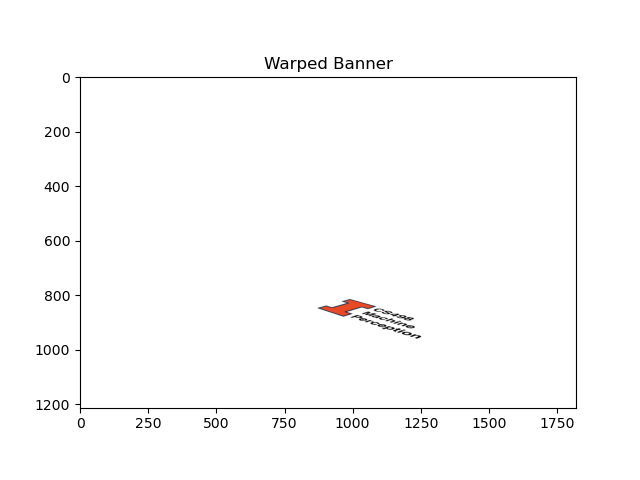
\includegraphics[width=8cm]{fig/warped_banner.png}
\end{center}


\item \textbf{3.c [1pt]:} alpha-blend the warped logo onto the court: $I = \alpha F + (1 - \alpha) B$

\textbf{Answer}: Here I set alpha logo to be 0.8 and use the following codes to solve the problem of uneven transparency.

\begin{figure}[htbp]
    \small
    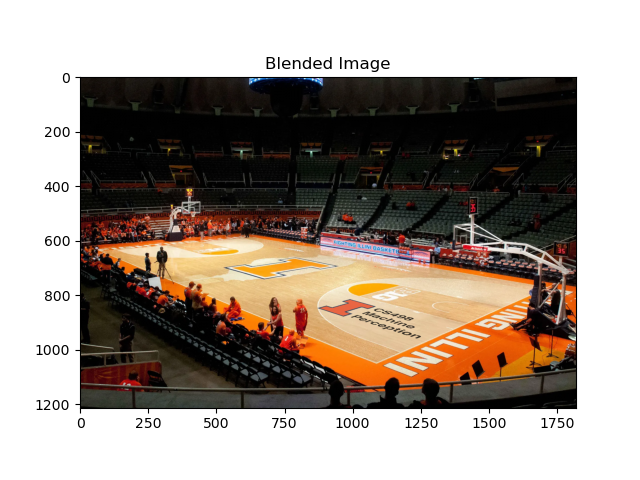
\includegraphics[width=0.48\linewidth]{fig/blended_image.png}
    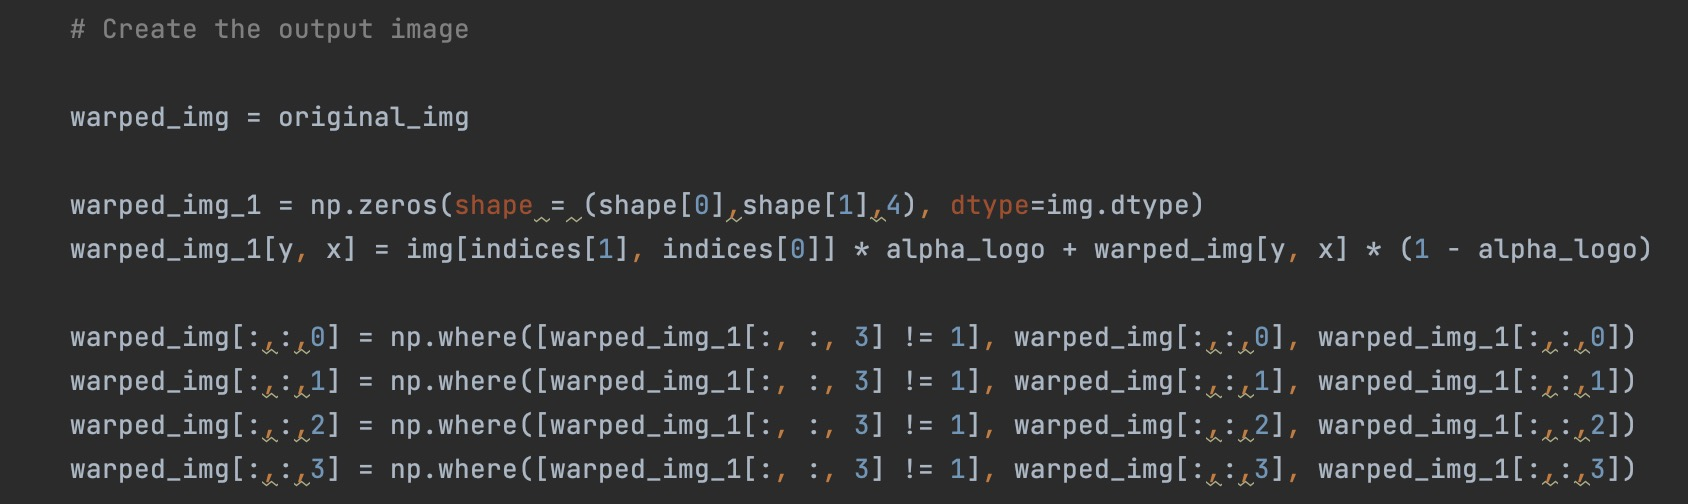
\includegraphics[width=0.6\linewidth]{fig/codes.png}
\end{figure}

\end{itemize}



\section*{Perspective Projection [7pts]}
Till now we have been working on transformations between 2D coordinate systems. Now let us to lift up to the 3D coordinate. Consider the same image of the state farm center, but this time, we annotate four additional points, corresponding to the four corners of the basketball backboard. 

\paragraph{Question 4 [1pt]:} 
The lower rim of the backboard is 2.745 meters above the ground; the backboard width is 1.83 meters and backboard height is 1.22 meters. The backboard protrudes 1.22 meters out from the baseline. Now let us consider the world frame. The world frame coordinate origin is at the point \#3, where x-axis is along the long edge (sideline) and y-axis is along the short edge (baseline), and z-axis is upwards, perpendicular to the basketball court.   Could you compute the 3D coordinates of all the eight keypoints?

\textbf{Answer}: The 3D coordinates of all eight keypoints in non-homogeneous are shows as follows, each row represents a keypoint:

\[ eight points = 
\left[
\begin{array}{ccc}
    0 & court width & 0 \\
    court length & court width & 0 \\
    court length & 0 & 0 \\
    0 & 0 & 0 \\
    board to baseline & (court width - backboard width)/2 & lower rim + backboard height\\
    board to baseline & (court width + backboard width)/2 & lower rim + backboard height\\
    board to baseline & (court width + backboard width)/2 & lower rim\\
    board to baseline & (court width - backboard width)/2 & lower rim\\
\end{array}
\right] \]
\\
\[= 
\left[
\begin{array}{ccc}
    0 & 15.24 & 0 \\ 
    28.65 & 15.24 & 0 \\
    28.65 & 0 & 0 \\
    0 &  0 & 0 \\ 
    1.22 & 6.705 & 3.965 \\ 
    1.22 & 8.535 & 3.965 \\ 
    1.22 & 8.535 & 2.7449999999999997 \\ 
    1.22 & 6.705 & 2.7449999999999997\\
\end{array}
\right]
\]

\paragraph{Question 5 [4pt]:} 
Now we have established eight pairs of 2D and 3D keypoint correspondences. 
Consider this set of correspondence pairs in homogeneous coordinates $(\mathbf{x}_i, \mathbf{X}_i)$. Our goal is to compute a perspective projection matrix such that: 
\[
\mathbf{x}_i = \alpha \mathbf{P} \mathbf{X}_i = 
\alpha \left[
\begin{array}{c}
\mathbf{p}_1^T \\
\mathbf{p}_2^T \\
\mathbf{p}_3^T
\end{array}
\right]
\mathbf{X}_i
= 
\alpha \left[
\begin{array}{c}
\mathbf{p}_1^T\mathbf{X}_i \\
\mathbf{p}_2^T\mathbf{X}_i \\
\mathbf{p}_3^T\mathbf{X}_i
\end{array}
\right]
\]
where $\mathbf{p}_i^T$ is the $i$th row of $\mathbf{P}$; $\mathbf{x}_i = (x_i, y_i, 1)^T$; $\alpha$ is an arbitrary scalar. 

\begin{itemize}
\item \textbf{5.a [1pt]:} Please prove that:
\[
\mathbf{A}_i 
\left[
\begin{array}{c}
\mathbf{p}_1 \\
\mathbf{p}_2 \\
\mathbf{p}_3
\end{array}
\right] = \mathbf{0} \textrm{\ where \ } \mathbf{A}_i = \left[
\begin{array}{ccc}
\mathbf{0} & \mathbf{X}_i^T & - y_i \mathbf{X}_i^T \\
\mathbf{X}_i^T & \mathbf{0} & - x_i \mathbf{X}_i^T \\
\end{array}
\right].
\]

\textbf{Answer}: Since we know that 
\[
\mathbf{x}_i = \alpha \mathbf{P} \mathbf{X}_i
\]

$\alpha$ here represents scalar ambiguity, so we can put it into x,y coordinate and write it as 
\[
\mathbf{x}_i^{\star} = \mathbf{P} \mathbf{X}_i
\]

which can be written as follows:
\[
\begin{array}{c}
    {\left[\begin{array}{l}
    \frac{x}{\alpha} \\
    \frac{y}{\alpha} \\
    \frac{z}{\alpha}
    \end{array}\right]=\left[\begin{array}{lll}
    h_{1} & h_{2} & h_{3} \\
    h_{4} & h_{5} & h_{6} \\
    h_{7} & h_{8} & h_{9}
    \end{array}\right]\left[\begin{array}{c}
    X \\
    Y \\
    1
    \end{array}\right]} \\
\end{array}
\]

which can be written as follow after normalized:
\[
    x^{\prime}=\frac{h_{1} X+h_{2} Y+h_{3}}{h_{7} X+h_{8} Y+h_{9}} \quad y^{\prime}=\frac{h_{4} X+h_{5} Y+h_{6}}{h_{7} X+h_{8} Y+h_{9}}    
\]

\[
\begin{array}{c}
    h_{1} X+h_{2} Y+h_{3}-x^{\prime}\left(h_{7} X+h_{8} Y+h_{9}\right)=0 \\
    h_{4} X+h_{5} Y+h_{7}-y^{\prime}\left(h_{7} X+h_{8} Y+h_{9}\right)=0
\end{array}
\]

which can be written into matrix multiplication form as follows:
\[
\left[\begin{array}{ccccccccc}
    0 & 0 & 0 & X & Y & 1 & -y^{\prime} X & -y^{\prime} Y & -y^{\prime} \\
    X & Y & 1 & 0 & 0 & 0 & -x^{\prime} X & -x^{\prime} Y & -x^{\prime}
    \end{array}\right]\left[\begin{array}{c}
    h_{1} \\
    h_{2} \\
    h_{3} \\
    \cdots \\
    h_{9}
\end{array}\right]=0    
\]

which is equal to:
\[
\mathbf{A}_i 
\left[
\begin{array}{c}
\mathbf{p}_1 \\
\mathbf{p}_2 \\
\mathbf{p}_3
\end{array}
\right] = \mathbf{0} \textrm{\ where \ } \mathbf{A}_i = \left[
\begin{array}{ccc}
\mathbf{0} & \mathbf{X}_i^T & - y_i \mathbf{X}_i^T \\
\mathbf{X}_i^T & \mathbf{0} & - x_i \mathbf{X}_i^T \\
\end{array}
\right].
\]


\item \textbf{5.b [3pt]:} complete the \texttt{findProjection} function and use this function to recover the perspective camera projection matrix, from the 3D world coordinate to the 2D image coordinate. Hints: 1) establish a linear system based on your derivation 2) given the eight keypoint correspondences, how many equations and how many unknown variables? 3) consider using \texttt{numpy.linalg.svd} to solve the linear system. 4) you might find \texttt{numpy.concatenate} and \texttt{numpy.reshape} to be handy.  

\textbf{Answer}: The projection matrix is shown as follows:

projection matrix = 
\[
\left[
\begin{array}{cccc}
    1.18682798e+01 & 5.03681893e+01 & 1.45686779e+01 & 7.34119776e+01 \\
    -8.26855706e+00 & 8.76915144e+00 & -2.39149474e+01 & 6.35921983e+02 \\ 
    -2.16285953e-02 & 2.02166814e-02 & 4.33368607e-02 & 1.00000000e+00 \\
\end{array}
\right]
\]

And the reporjection result is shown as follows:

\begin{center}
    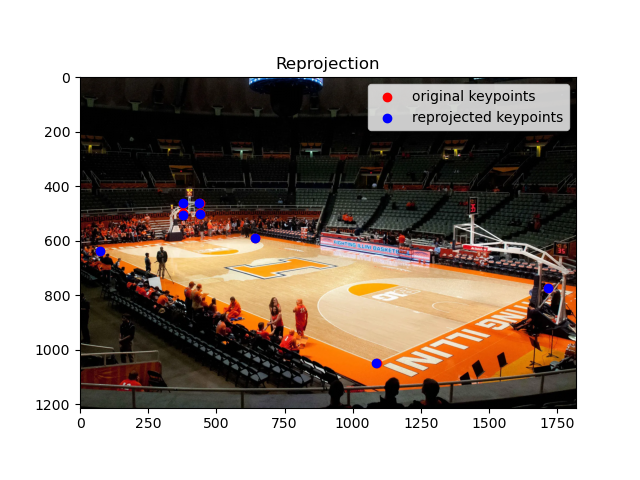
\includegraphics[width=8cm]{fig/reprojection.png}
\end{center}

\item \textbf{5.c [1pt bonus]:} Try to answer the following questions: 1) assuming perfect correspondences, could we recover the projection matrix using even fewer points? Please indicate how many correspondences at least we need. 2) could we just use correspondences on the ground plane to recover this projection matrix? Please explain why or why not.     

\textbf{Answer}: 1) The projection matrix needs at least 6 points to recover. This is because with 6 correspondences, we can construct a system of 12 equations and solve for the 12 unknown variables in the projection matrix. Any fewer correspondences would result in an underdetermined system.

2) we cannot just use correspondences on the ground plane to recover the projection matrix. This is because we need data from all three dimensions to recover the projection matrix. To be specific, if we only have correspondences on the groud plane, its z-value will be 0, which means we can not determine the value of $p_3$, $p_7$ and $p_11$ in the projection matrix.

\end{itemize}

\paragraph{Question 6 [2pt]:}
Using our estimated projection matrix in Q5, we could insert any 3D object in the world coordinate frame onto the 2D image. In this question, let's consider the a simple case where we want to project a 3D point cloud onto the image plane and plot them. Suppose we want to put a giant stanford bunny statue in the center of the basketball court, could you compute the 2D coordinate of every vertex of this bunny using the projection matrix? Hints: 1) you might need to transform the bunny to the court center first 2) make sure the bunny is above the ground. 

\textbf{Answer}: Firstly I centralize the 3D object in its x-axis and y-axis to 0 and add half of the court length and half of the court width to first channel and second channel (x direction and y direction) of each verts respectively to put the bunny to the center of the court and minus each pixels' third channel value with the smallest value for all pixels in the third channel (z-direction) to put the bunny above the ground.Then I use projection matrix to project 3-d points into 2-d image.

The projection result of stanford bunny statue is shown as follows:

\begin{center}
    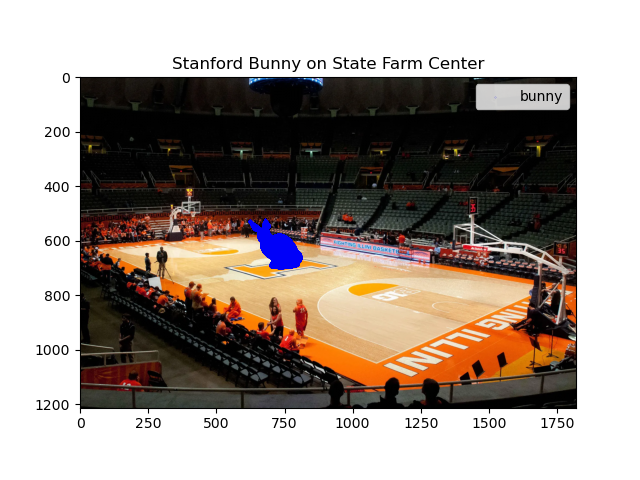
\includegraphics[width=8cm]{fig/stanfordbunnyonstatefarmcenter.png}
\end{center}

\paragraph{Question 7 [2pt bonus]:} Try to use an off-the-shelf renderer to render the 3D mesh in a more realistic manner (e.g. pyrender, moderngl, blender, mitsuba2). You could consider the following aspects that might influence the realism: 1) shading 2) shadows 3) occlusion reasoning 4) lighting environments. 

Hints: for some libraries, you probably need to decompose the projection matrix into valid intrinsic and extrinsic matrices. You can also manually annotate additional key points to make the projection matrix estimation more accurate in this experiment.

\textbf{Answer}: I use pyrender to render the 3D mesh. Firstly I centralize the 3D points in x and y direction, then I use mesh.frompoints to transform 3D coordinates into mesh items. After that, I set scene, light parameter and choose orthographic camera. The position of light and scene is same to mesh coordinate. The camera coordinate system is rotated firstly around x-axis by $\pi/4$ and then around z-aixs by $\pi/4$. The result is shown as follow, The left one is generated by only vertices and the right one is generate by both vertices and faces: 

\begin{center}
    \small
    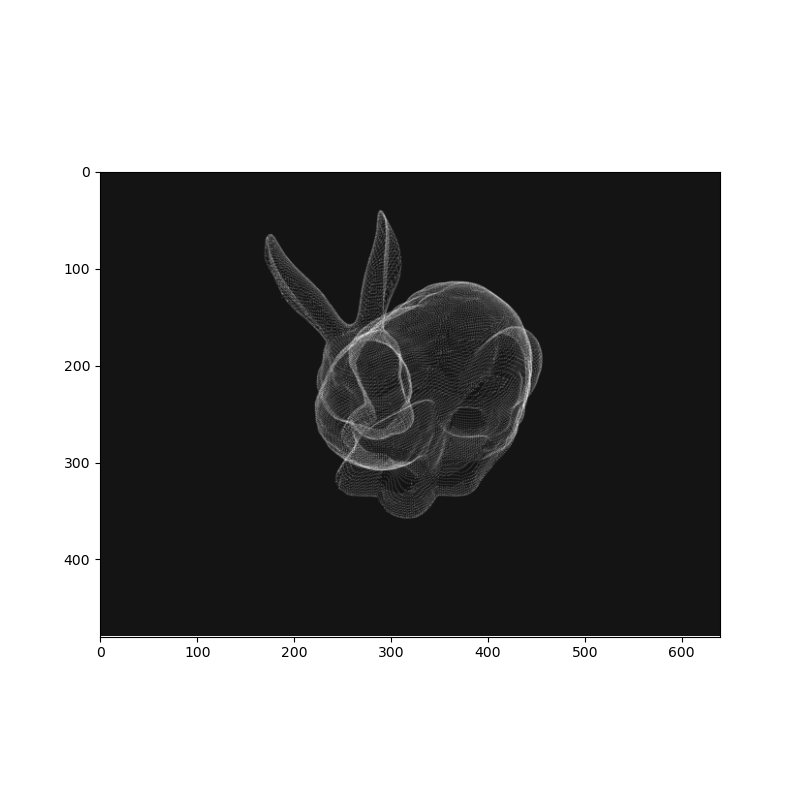
\includegraphics[width=0.37\linewidth]{fig/bunny_after_render.png}
    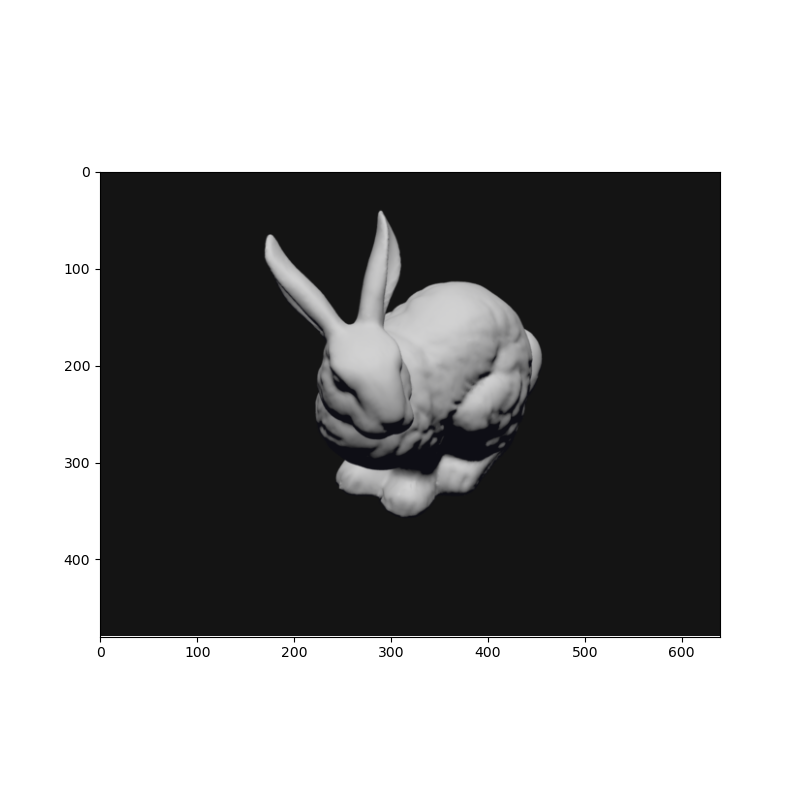
\includegraphics[width=0.37\linewidth]{fig/render_stanford_final.png}
\end{center}

\end{document}
\grid
\grid